\documentclass[tikz,border=2pt]{standalone}
\usepackage{amsmath}
\usepackage{pgfplots}
\pgfplotsset{compat=1.18}
\usetikzlibrary{arrows.meta}
\begin{document}
% f(x)=x_1x_2 on (0,inf)^2: level curves x_1x_2=1,4,9; the superlevel set {f>=4} (shaded) lies above the hyperbola
% x_2=4/x_1 and is convex, so f is quasi-concave. Not concave: f(2,2)=4 < 5 = average of f(1,1)=1 and f(3,3)=9.
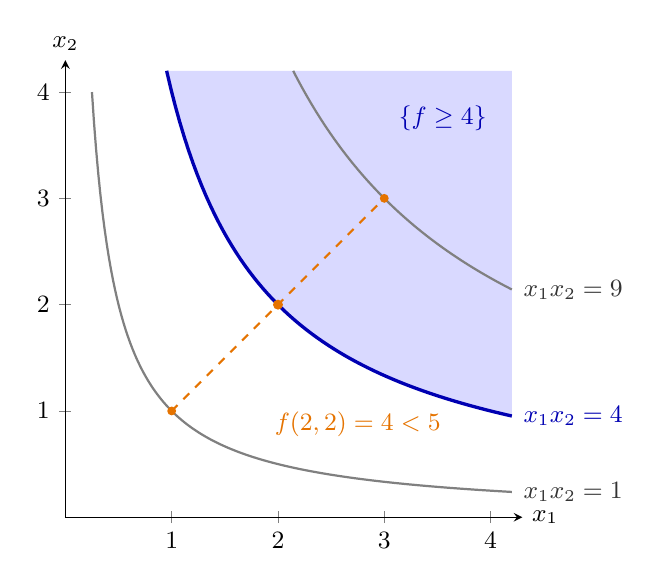
\begin{tikzpicture}[font=\small, >={Latex[length=2mm]}]
  \begin{axis}[
    axis lines=left, xmin=0, xmax=4.3, ymin=0, ymax=4.3,
    xtick={1,2,3,4}, ytick={1,2,3,4},
    xlabel={$x_1$}, ylabel={$x_2$},
    xlabel style={at={(axis description cs:1,0)}, anchor=west},
    ylabel style={rotate=-90, at={(axis description cs:0,1)}, anchor=south},
    x=1.35cm, y=1.35cm, clip=false
    ]
    \addplot[draw=none, fill=blue!15, domain=0.9524:4.2, samples=80] {4/x} -- (axis cs:4.2,4.2) -- cycle;
    \addplot[gray, thick, domain=0.25:4.2, samples=200] {1/x};
    \addplot[blue!70!black, very thick, domain=0.9524:4.2, samples=80] {4/x};
    \addplot[gray, thick, domain=2.1429:4.2, samples=80] {9/x};
    \node[gray!40!black, anchor=west] at (axis cs:4.22,0.24) {$x_1x_2=1$};
    \node[blue!70!black, anchor=west] at (axis cs:4.22,0.95) {$x_1x_2=4$};
    \node[gray!40!black, anchor=west] at (axis cs:4.22,2.14) {$x_1x_2=9$};
    \node[blue!70!black] at (axis cs:3.55,3.75) {$\{f\geq4\}$};
    \draw[orange!90!black, thick, dashed] (axis cs:1,1) -- (axis cs:3,3);
    \fill[orange!90!black] (axis cs:1,1) circle (1.6pt);
    \fill[orange!90!black] (axis cs:3,3) circle (1.6pt);
    \fill[orange!90!black] (axis cs:2,2) circle (1.8pt);
    \node[orange!90!black] at (axis cs:2.75,0.87) {$f(2,2)=4<5$};
  \end{axis}
\end{tikzpicture}
\end{document}
